\documentclass[a4paper]{memoir}
\usepackage[utf8]{inputenc}
\usepackage[frenchb]{babel}
\usepackage{graphicx}
\usepackage{float}
\usepackage{hyperref}
\usepackage{verbatim}
\usepackage{enumitem}

\pagestyle{plain}

\title{\textbf{Rapport de projet}\\- \Huge{Incidence} -}
\author{\emph{CHAMBONNET Kevin}\\\emph{GAUTHIER Silvère}\\\emph{MARTINEZ Thierry}\\\emph{MOKHRETAR Amin}}
\date{\today}

\begin{document}
	\maketitle
	\newpage
	\tableofcontents

	\chapter{Remerciements}

		Un grand merci à Fabien Hervouet pour son encadrement.
		Merci à Monsieur FERBER qui nous a orientés dans la réalisation du moteur multi-agent.

	\chapter{Introduction}
	
		\section{Philosophie}
			Du point de vue d’un observateur, un monde peut être qualifié de complexe sans que les individus y évoluant ne le soient forcément. Dans ce TER, il est question d’aborder cette thématique sous forme de jeu. Autrement dit, le problème qui nous intéresse ici est de déterminer comment faire émerger un comportement global en mettant en oeuvre des contraintes extérieures dans l’environnement pour influencer les interactions locales d’agents. De plus il faudra, pour le joueur, analyser le comportement des ces derniers afin d’optimiser la réalisation des buts demandés. Plus précisément, il s’agit de mettre en scène des agents (disposant d’un comportement précis et défini en terme d’interaction), évoluant dans un environnement modifiable par un joueur humain (qu’il s’agisse d’ajouter des ressources exploitables, de modifier le relief, etc.) devant atteindre un certain objectif (stabilité du système écologique, récolte d’une certaine quantité de ressources, développement d’un chemin).
		
		\section{Influences}
			Nous souhaitions avant tout réaliser un projet de jeux vidéos intégrant les notions de programmation multi-agent vues au semestre précédent, tout en implémentant notre propre version de moteur multi-agent. En effet, l'autonomie et l'indépendance des entités, en terme de comportement, étaient primordiales de notre point de vue. De plus, plusieurs jeux vidéos ont orienté la conception de notre projet, principalement From Dust par rapport à la possibilité de modifier l'environnement et les répercussions, mais aussi Age Of Empire II pour ce qui concerne la gestion des ressources et leur récolte. 
		
		\section{Sujet}
			Ce travail impliquera de s’intéresser au paradigme de la programmation multi-agents. À partir d’une plateforme existante (type TurtleKit) ou d’une version simple programmée pour l’occasion, on proposera différents niveaux de jeu qui offriront par exemple : (1) la possibilité de modifier l’environnement permettant, en terme de contraintes, d’insuffler une dynamique globale aux agents pour les mener à réaliser un certain but ; (2) la possibilité de modifier le comportement local des agents pour atteindre des buts plus complexes. 
			Le cadre plus précis sera à déterminer en fonction de faisabilités et des envies des étudiants : quelles actions pourront effectuer les agents ? quelles ressources à disposition ? quels types d’objectifs pour le joueur ? comment envisager la progression des niveaux ? D’autres évolutions sont possibles et seront traitées en fonction de l’avancement du projet : systèmes d’évènements (épidémies, catastrophe naturelle), outils simple pour la création de nouveaux niveaux, mode multi-joueurs, etc. 
			D’un point de vue pragmatique on s’attachera en priorité à étudier l’adéquation de la mise en oeuvre des comportements réactifs des agents face aux différentes possibilités de contraintes permises pour le joueur, ainsi qu’à l’ergonomie de l’interface. L’aspect recherche de ce TER se concentrera sur une familiarisation plus en profondeur avec le domaine de la modélisation et de la simulation multi-agents [1] ainsi qu’avec les méthodologies de conception de jeu [2].
	
	\chapter{Cahier des charges}
		Ce chapitre détaille toute la phase de conception du projet. Elle contient le Game Design Document que nous avons rédigé lors de l'étude préalable.
	
		\section{Questions fréquentes}
			Cette partie regroupe les caractéristiques basiques du jeu sous forme de questions-réponses.
		
			\subsection{Qu'est-ce que ce jeu ?}
				C'est un jeu de type God-Like dans lequel on doit aider une civilisation à survivre le plus longtemps possible grâce à différents pouvoirs et actions divines.
		
			\subsection{Qu'est-ce que je contrôle ?}
				Vous ne contrôlez rien directement, tout se fait de façon indirecte grâce aux pouvoirs. Modifier l'environnement et aider les citoyens sont des actions qu'il faudra effectuer pour faire survivre la civilisation.
	
			\subsection{Quelles sont les conditions de victoire et de défaite ?}
				Il n'y aura pas de condition de victoire particulière dans le jeu de base, le but sera de survivre le plus longtemps possible.\\
				La partie se terminera quand le joueur n'aura plus de citoyen.
			
		\section{Mecanismes de jeu}
			Cette section détaille succintement les possibilités du joueur pendant la partie.
			
			\subsection{Les Pouvoirs}
				\label{Pouvoirs}
				Le joueur aura la possibilité d'interagir sur l'environnement via differents pouvoirs.
				
				\begin{itemize}[label=$\bullet$]
					\item \textbf{Placer un Arbre :} Fait apparaître un Arbre sur une case choisie. Coût : 3 PI.
					\item \textbf{Placer un Arbre Fruitier :} Fait apparaître un Arbre Fruitier sur une case choisie. Coût : 6 PI.
					\item \textbf{Placer de la Pierre :} Fait apparaître de la Pierre sur une case choisie. Coût : 5 PI.
					\item \textbf{Placer de l'Eau :} Fait apparaître de l'Eau sur une case choisie. Coût : 2 PI.
					\item \textbf{Placer une Falaise :} Fait apparaître une Falaise sur une case choisie. Coût : 7 PI.
					\item \textbf{Placer un Buisson :} Fait apparaître un Buisson sur une case choisie. Coût : 4 PI.
					\item \textbf{Placer de la Terre :} Fait apparaître de la Terre sur une case choisie, la Terre placée s'adapte en fonction des autres Terres autour. Coût : 2 PI.
				\end{itemize}
				\begin{itemize}[label=$\bullet$]
					\item \textbf{Soigner :} Améliore l'état de santé d'un citoyen. Coût : 50 PI.
					\item \textbf{Naissance :} Crée un citoyen supplémentaire, hors naissances quotidiennes. Coût : 200 PI.
				\end{itemize}

			\subsection{Choix de la nuit}
				Lors de la partie, il y aura plusieurs phases de jeu : le jour et la nuit. Chaque jour, le joueur peut effectuer les actions ci-dessus, et lors de la nuit, il a la possibilité de définir des paramètres pour le jour suivant :
				\begin{itemize}[label=$\bullet$]
					\item \textbf{Météo :} Le joueur peut choisir la météo du jour suivant (ensoleillée ou pluvieuse).
					\item \textbf{Métier :} Le joueur peut orienter la distribution des métiers, sans définir exactement la proportion de chaque métier.
				\end{itemize}
		
			\subsection{Sauver et Charger une partie}
				Le joueur pourra sauvegarder sa partie à tout moment, mais la sauvegarde se fera au moment de la dernière nuit.\\
				Le chargement d'une partie placera donc le joueur soit au début de la partie soit à la dernière nuit passée, avec la possibilité de modifier de nouveau les différentes options du jour (météo, métiers...).
	
		\section{Structure du jeu}
			Cette partie détaille succintement la structure globale du jeu, ce qui couvre les aspects du jeu non maîtrisables par le joueur.
			
			\subsection{Moteur multi-agent}
				La gestion multi-agent se fera à l'aide d'un appel au script de chaque catégorie d'entité pour chaque tick. Chaque catégorie d'entité aura donc un script propre, qui décrira son comportement et pourra faire appel aux primitives que fournira le moteur pour decider de l'action à faire.
				\subsubsection{Primitives}
					Toutes les primitives seront des informations accessibles par les entiés dans leur script. Ci-dessous une liste des primitives les plus importantes.
					\begin{itemize}[label=$\bullet$]
						\item Connaître les entités et cases alentours
						\item Connaître l'emplacement du village
						\item Changer de direction
						\item Connaitre sa santé
						\item Si leur sac est plein
						\item S'il est attaqué
						\item Par qui sont-ils attaqué
					\end{itemize}
			
			
				\subsubsection{Actions}
					Les actions principales des entités seront predefinis, le script devra retourner une action pour que l'entités agissent. Ci-dessous la liste de ces actions.
					\begin{itemize}[label=$\bullet$]
						\item Avancer
						\item Couper un Arbre
						\item Ramasser des Baies
						\item Casser de la Pierre
						\item Rentrer au village
						\item Attaquer une entité
					\end{itemize}


			\subsection{Les Entites}
				Les Entites sont tout les elements mobiles du jeu. Il y aura différent groupe d'entites, les citoyens seront les entités du joueur, il y aura aussi des animaux et des citoyens ennemis.

				\subsubsection{Les métiers des citoyens}
					\label{Metier}
					Chaque citoyen aura une tâche à accomplir durant la journée et ne pourra pas en changer avant la nuit. La nuit, un métier sera attribué à chaque citoyen selon les choix du joueur et les besoins des citoyens (cf. section \ref{Cycle}, page \pageref{Cycle}).
					\begin{itemize}[label=$\bullet$]
						\item \textbf{Bûcheron :} Coupe les arbres et récolte les ressources associées (Le Bois en général mais aussi de la nourriture sur les Arbres Fruitier).
						\item \textbf{Mineur :} Casse les rochers et récolte la Pierre.
						\item \textbf{Chasseur-Cueilleur :} Chasse les animaux, cueille les baies ou cultive des champs pour récolter la Nourriture.
					\end{itemize}

				\subsubsection{La santé des entités vivantes}
					Chacune des entités possède une gestion de la santé avec plusieurs états.
					\begin{itemize}[label=$\bullet$]
						\item \textbf{Bonne santé :} Si l'entité est un citoyen, elle offre de plus grands bonus de PI.
						\item \textbf{Normal :} L'entité est dans son état par défaut.
						\item \textbf{Blessé/Malade :} L'entité agit avec un léger malus de vitesse. Si l'entité est un citoyen, elle offre de plus petits bonus de PI.
						\item \textbf{Gravement blessé/malade :} L'entité agit avec un malus de vitesse plus important. Si l'entité est un citoyen, elle n'offre plus de PI.
						\item \textbf{Mort :} L'entité disparaît.
					\end{itemize}
					\begin{figure}[H]
						\begin{center}
							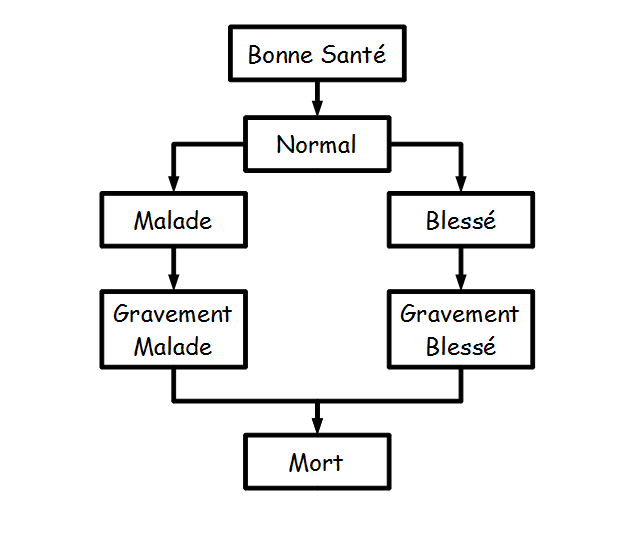
\includegraphics[scale=0.5]{img/DiagrammeTransitionSante.png} 
						\end{center}
						\label{fig:sante}
						\caption{Diagramme de transitions entre les états de santé}
					\end{figure}
	
			\subsection{Moteur de carte}
				La gestion de la carte se fera uniquement en c++. Il existera pour cela différentes classes comme TileMap, Ground, Element et Tileset.
		
				\subsubsection{La carte}

					La carte sera composée de 150x150 cases, mais ne sera affiché à l'écran qu'une vingtaine de cases en largeur sur une quinzaine en hauteur. Le déplacement sur la carte pourra se faire grâce aux touches fléchées mais aussi en plaçant la souris sur un des bords de l'écran.\\
					Le joueur ne pourra pas voir au delà des limites des 150x150 cases composant la carte.

				\subsubsection{Les Cases}

					La carte sera découpée en cases. Chaque case aura un type de base en début de partie, qui pourra ensuite être modifié selon le déroulement du jeu (cf. figure \ref{fig:case}, page \pageref{fig:case}). Un élément neutre est un type de case ne donnant pas lieu à une ressource quelconque.\\
					\\
					\begin{table}[H]
						\begin{small}
							\begin{tabular}{| c | c | c |p{5cm}|}
								\hline
								&    &    &    \\
								\textbf{Type de case} & \textbf{Ressources} & \textbf{Franchissable} & \textbf{Description}\\
								&    &    &    \\
								\hline
								Terre & - & Oui & Type par défaut.\\
								\hline
								Terre Aride & - & Oui & Terre ne pouvant pas être cultivée.\\
								\hline
								Terre Innondée & - & Oui & Terre ne pouvant pas être cultivée.\\
								\hline
								Terre Fertile & - & Oui & Terre pouvant etre cultivée pour devenir un \textbf{Champs}.\\
								\hline
								Champs & Nourriture & Oui & Terre cultivée possédant plusieurs stades de maturité. Le maximum atteint, la récolte peut être effectuée et offrir de la nourriture.\\
								& (1 à 3 unités) &    &    \\
								\hline
								Arbre & Bois & Non & Peut être coupé pour récolter du bois.\\
								& (3 unités) &    &    \\
								\hline
								Arbre Fruitier & Bois, Nourriture & Non & Peut être coupé pour récolter du bois et de la nourriture.\\
								& (2 unités de chaque) &    &    \\
								\hline
								Eau & - & Non & Des poissons peuvent s'y trouver permettant de récolter de la nourriture.\\
								\hline
								Pierre & Pierre & Non & Peut être cassée pour récolter de la pierre.\\
								& (2 unités) &    &    \\
								\hline
								Falaise & - & Non & Elément neutre. Peut faire apparaître de la pierre à ses pieds.\\
								\hline
								Buisson & Nourriture & Non & La récolte de ses baies permet d'obtenir de la nourriture.\\
								& (2 unités) &    &    \\
								\hline
							\end{tabular}
						\end{small}
						\label{tab:case}
						\caption{Les différents types de case}
					\end{table}
		
				\subsubsection{Diagramme de transitions des différentes cases}
					Chaque type de case est compatible avec d'autres types. Les transitions entre les types sont détaillées dans ce diagramme :
					\begin{figure}[H]
						\begin{center}
							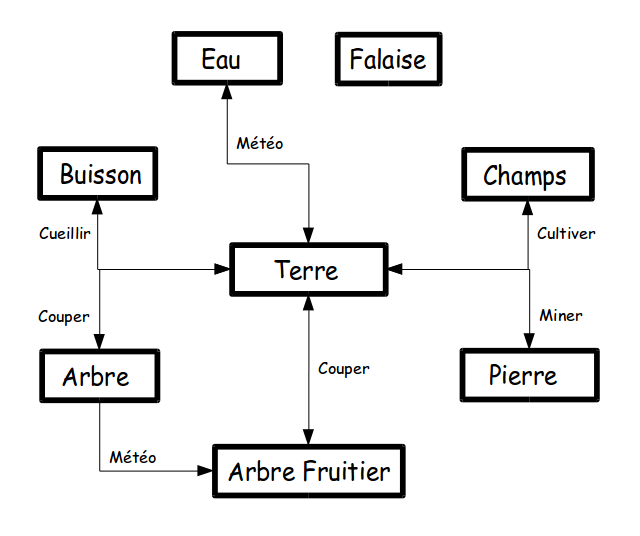
\includegraphics[scale=0.35]{img/DiagrammeTransitionCases.png} 
						\end{center}
						\label{fig:case}
						\caption{Diagramme de transitions entre les types de case}
					\end{figure}
			
				\subsubsection{Les incidences sur l'environnement :}
					Lors de la nuit, les actions de la journée ont ce que l'on appelle des incidences sur les journées suivantes, c'est-à-dire des conséquences soit bénéfiques, soit néfastes. Par exemple :
					\begin{itemize}[label=$\bullet$]
						\item Une étendue d'eau peut faire apparaître des poissons.
						\item Une étendue d'eau peut faire apparaître de la végétation dans les environs.
						\item Une zone de végétation très dense augmente les chances de faire apparaître des animaux herbivores.
						\item Une grande concentration d'animaux herbivores peut faire apparaître des animaux carnivores.
						\item Une forêt très dense augmente les chances de faire apparaître des arbres fruitiers.
						\item Les falaises peuvent faire apparaître des pierres par éboulement.
						\item La météo peut modifier la taille des étendues d'eau, assécher ou humidifier la terre.
					\end{itemize}
				
				
			\subsection{Les Ressources}
				Différentes ressources telles que le bois, la pierre ou la nourriture seront disponibles sur la carte, et d'autres comme les "points d'incidence", seront générées au cours de la partie.
				
				\subsubsection{Ressources utilisées par les citoyens}
					Ces ressources pourront être stockées dans une quantité illimitée, et les citoyens les utiliseront pour des constructions ou pour se nourrir.
					\begin{itemize}[label=$\bullet$]
						\item \textbf{Bois :} Utilisé pour la construction des bâtiments.
						\item \textbf{Pierre :} Utilisé pour la construction de certains bâtiments.
						\item \textbf{Nourriture :} Consommé par les citoyens chaque nuit pour se nourrir.
					\end{itemize}
					\textbf{Comment ces ressources sont-elles récoltées ? }\\
					Elles sont récoltées par les citoyens, ainsi chaque métier correspond à la récolte d'une de ces ressources (cf. section \ref{Metier}, page \pageref{Metier}).

				\subsubsection{Ressources utilisées par le joueur}
					Cette ressource est la seule que le joueur pourra utiliser, elle sera stockée dans une quantité illimitée.
					\begin{itemize}[label=$\bullet$]
						\item \textbf{Point d'Incidence (PI) :} Utilisé à chaque action ou pouvoir divin.
					\end{itemize}
					\textbf{Comment cette ressource est-elle récoltée ? }\\
					Elle sera obtenue grâce aux citoyens qui nous en feront gagner une petite quantité tout au long de leur journée. La nuit, chaque citoyen rapporte des points bonus.

			\subsection{La météorologie}
				La météo sera présente et sera contrôlée par le joueur. Elle aura une incidence sur l'environnement et les citoyens. Elle sera basique : ensoleillée ou pluvieuse, chacune des deux aura une incidence différente. 
				\begin{itemize}[label=$\bullet$]
					\item \textbf{Temps ensoleillé :} Améliore la pousse des champs mais un excès de soleil assèche les terres et récoltes, peut réduire les étendues d'eau et une sécheresse trop longue peut faire brûler certaines ressources.
					\item \textbf{Temps pluvieux :} Permet de faire pousser les champs. Un surplus de pluie innonde les terres et récoltes, augmente les probabilités de maladie et peut augmenter la taille des étendues d'eau.
				\end{itemize}


			\subsection{Le cycle jour/nuit}
				\label{Cycle}
				Un cycle jour/nuit sera présent, avec des journées longues et des nuits courtes. Le Jour, les citoyens se vouent à leur métier, jusqu'au soir. La Nuit, tous les citoyens retournent au village, plus aucune action n'est possible. Lorsque la nuit tombe, toutes les actions du jour ont une incidence sur la nature et les entités, et seront visibles au début de la nouvelle journée.
				\begin{itemize}[label=$\bullet$]
					\item Le terrain est mis à jour, toutes les actions de la journée auront une incidence sur l'environnement.
					\item Tous les citoyens se nourrissent, la nourriture diminue en fonction du nombre de citoyen \textit{(-3 de nourriture par citoyen)}. S'ils manquent de la nourriture, certains citoyens peuvent tomber malade.
					\item Certains citoyens tombent malade en fonction des anciennes météos.
					\item S'il y a assez de nourriture, de nouveaux citoyens peuvent naître.
					\item Gain des points bonus d'incidence en fonction de la taille de la population et de sa santé.
					\item Mise à jour du métier de chaque citoyen, choisi en fonction des choix du joueur et des besoins.
				\end{itemize}

			\subsection{Scripts}
				Chaque catégorie d'entités déterminée selon leur classe d'appartenance aura un script propre. Ce script sera appelé à une fréquence variable en fonction de la situation dans laquelle se trouvera l'entité.
			
		\section{Eléments graphiques}
			Tous les effets graphiques du projet sont à base de sprites. Nous avons initialement choisi des tuiles de 32x32 pixels, mais il serait possible de changer cette taille dans le futur.\\

			\subsection{Les tuiles}
				\label{Tuile}
				Les tuiles seront des images de 32x32 ou 16x16 pixels au format PNG.\\
				\begin{itemize}[label=$\bullet$]
					\item \textbf{Le sol :} Il y aura 16 tuiles pour chaque type de sol, correspondant à toutes les possibilités de jonction avec le type voisin. En effet, chaque type de sol ne pourra être en contact qu'avec deux types différents suivant l'ordre hiérarchique suivant :\\
					Eau $\rightarrow$ Terre innondée $\rightarrow$ Terre fertile $\rightarrow$ Terre $\rightarrow$ Terre aride
					\item \textbf{Les ressources :} Il y aura 4 tuiles pour chaque ressource, correspondant au type de sol sur lequel elle se trouve.
					\item \textbf{Les bâtiments :} Chaque bâtiment sera constitué d'un ensemble de tuiles.
				\end{itemize}
				Chaque sol du tileset est affiché avec des bordures selon les types de sols environnant.\\
				\begin{figure}[H]
					\begin{center}
						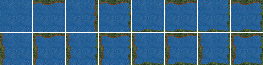
\includegraphics[scale=1]{img/groundSample.png}
					\end{center}
					\label{fig:groundSample}
					\caption{Exemple de sol avec différentes bordures}
				\end{figure}
				Chaque élément est affiché différemment selon le type de sol sur lequel il se trouve.\\
				\begin{figure}[H]
					\begin{center}
						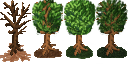
\includegraphics[scale=1]{img/elementSample.png}
					\end{center}
					\label{fig:elementSample}
					\caption{Exemple d'élément selon différents types de sol}
				\end{figure}
	
			\subsection{Les entités}
				Chaque entité aura plusieurs positions possibles. Pour chacun d'elle, un ou plusieurs éléments graphiques seront créés.\\
				\textbf{Les positions basiques :} Face, dos, profil droit, profil gauche.\\
				\textbf{Les positions spécifiques :} Coupant du bois, ramassant des baies, chassant, cultivant, construisant, se déplaçant sans ressource, se déplaçant avec des ressources.\\
				Chaque entité est animée selon sa classe, son sens de déplacement ou son action.\\
				\begin{figure}[H]
					\begin{center}
						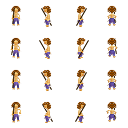
\includegraphics[scale=1]{img/animationSample.png}
					\end{center}
					\label{fig:animationSample}
					\caption{Exemple de fichier image pour une animation}
				\end{figure}
	
			\subsection{Interface utilisateur}
				Nous aurons différents menus, tels que menu principal, menu de jeu ou menu de la nuit. Ils auront chacun un certain nombre de boutons que nous ne détaillerons pas pour l'instant. Il y aura également un bandeau d'affichage des quantités de ressources pendant le jeu ainsi que des boutons permettant au joueur d'effectuer les actions utilisateur.
		
	\chapter{Gestion du projet}
		Cette partie traite globalement de tout ce qui concerne l'organisation du projet, que ce soit au niveau de la conception, du développement, de l'équipe ou encore de la gestion des fichiers.
		
		\section{Gestion de l'équipe}
			Tous les membres se connaissant et étant supposés être capable de travailler en équipe, nous n'avons fait aucune élection de chef de projet.\\
			Nous avons opté pour travailler de manière collégiale, et ainsi garder une cohésion de groupe sans pour autant avoir de hiérarchie instaurée au sein du groupe, qui pourrait au contraire déservir la réalisation de nos objectifs.\\
			Chaque membre a donc autant de pouvoir que les autres, et peut donc participer activement au projet, autant lors de la conception que du développement. Toutes les décisions seront prises suivant la majorité lors de votes.\\\\
			Pour ce qui est des réunions de projets, nous avons convenu avec notre tuteur d'une réunion, allant d'environ trente minutes à une heure, toutes les une à deux semaines, afin de mettre au point l'avancement du projet. En parallèle, tous les membres de notre équipe se retrouvent une fois par semaine afin de discuter des points clés effectués ou à venir, donner lieu aux votes pour les prises de décisions, ou encore, lors de la phase de développement, travailler en collaboration afin d'optimiser notre travail.\\\\
			Au niveau du travail collaboratif, nous avons mis en place un dépôt sur github, contenant tant la documentation telle que ce rapport que les sources de notre jeu. Par ailleurs, nous mettrons sur ce dépôt uniquement les fichiers sources, les images et les sons, mais en aucun cas les fichiers temporaires ou les exécutables. Un fichier "makefile" sera disponible pour quiconque voudrait compiler le programme chez lui. Les seuls fichiers binaires disponibles seront les PDF de la documentation, pour un soucis de facilité d'accès.

		\section{Découpage en tâches}
			Afin de préparer le développement du jeu, il était nécessaire de séparer les fonctionnalités les unes des autres. Nous avons abouti à ce diagramme, qui résume notre choix de découpage :\\
			\begin{figure}[H]
				\begin{center}
					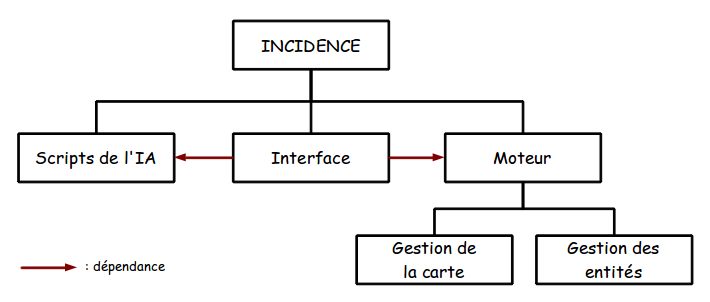
\includegraphics[scale=0.5]{img/DiagrammeDecoupageProjet.png}
				\end{center}
				\label{fig:decoupage}
				\caption{Diagramme des tâches du projet}
			\end{figure}

		\section{Assignation}
			Le projet étant maintenant découpé en un certain nombre de modules, il ne restait plus qu'à assigner chaque tâche à un ou plusieurs membres de l'équipe. Nous nous sommes organisés comme ceci :
			\begin{itemize}[label=$\bullet$]
				\item \textbf{Scripts de l'IA :} MARTINEZ Thierry, MOKHRETAR Amin.
				\item \textbf{Moteur :}
				\begin{itemize}[label=$\bullet$]
					\item \textbf{Gestion de la carte :} GAUTHIER Silvère.
					\item \textbf{Gestion des entités :} CHAMBONNET Kevin.
				\end{itemize}
				\item \textbf{Interface :} Tous les membres.
			\end{itemize}
			Bien entendu, cette répartition n'est pas totalement fixée, elle concerne en réalité l'affectation de responsables de parties, qui seront en charge de celle-ci mais pourront évidemment faire appel aux autres membres pour trouver une solution à un problème par exemple.\\
			Le détail complet des tâches et assignations se situe dans la section Gestion du temps, page \pageref{GestionTps}.

		\section{Gestion du temps}
			\label{GestionTps}
			Afin de clarifier notre gestion du temps, un diagramme de Gantt est disponible en annexe et dans la documentation de notre projet, et sera mis à jour en fonction de l'avancée du projet.\\

		\section{Profil de risques}
			Le profil de risque est là pour estimer la difficulte du projet dans different domaine.
	
			La taille est un des risque majeur de notre projet, n'ayant que 4 mois pour réaliser la totalité du projet, on a estimé ce temps très court par rapport à toutes les fonctionnalité qu'on souhaitait implémenter. D'où, une note de 5, sur ce point là.
			
			La difficulté technique est un point particulier vu que la grande majorité du projet etait facilement réalisable pour au moins une des personnes du groupe. Le projet ayant un but pédagogique, on s'est réparti les taches de manière à ce que chaque membre puisse travailler sur une partie qui lui ferait découvrir ou apprendre quelque chose. Ce qui apporte une certaines difficulté au projet.

			Le changement et l'instabilité de l'equipe sont les points les plus bas car notre equipe est constitué de personne ayant deja travaillé ensemble, on estime  donc que notre equipe sera stable et comme le projet est une idée de notre groupe, les changements seront des décisions prises par toutes l'equipe sauf de possible contrainte de notre encadrant.

			\begin{table}[H]
				\begin{small}
					\begin{tabular}{| c | l |}
						\hline
						\textbf{Nature du risque} & \textbf{Degré du risque pour le projet}\\
						& 0 \hspace{0.5cm} 1 \hspace{0.5cm} 2 \hspace{0.5cm} 3 \hspace{0.5cm} 4 \hspace{0.5cm} 5\\
						\hline
						Taille du projet & \hspace{4.5cm} \circle*{5}\\
						\cline{1-1}
						Difficulté technique & \hspace{2.7cm} \circle*{5}\\
						\cline{1-1}
						Degré d'intégration & \hspace{2.25cm} \circle*{5}\\
						\cline{1-1}
						Configuration organisationnelle & \hspace{1.8cm} \circle*{5}\\
						\cline{1-1}
						Changement & \hspace{0.9cm} \circle*{5}\\
						\cline{1-1}
						Instabilité de l'équipe de projet & \hspace{0.9cm} \circle*{5}\\
						\hline
					\end{tabular}
				\end{small}
				\label{tab:risk}
				\caption{Profil de risque du projet Incidence}
			\end{table}

Pour palier à notre problème de taille, on a rapidement mis en place un ordre de priorité sur les differentes fonctionnalités. On a dans un premier temps defini un noyau central qui définira le contenu minimum du projet, puis un ordre sur toutes les ordres fonctionnalités.

		\section{Choix technologiques}
			Afin de pouvoir développer correctement notre logiciel, il a fallu définir tout ce que nous allions utiliser en terme de langages et bibliothèques selon notre logique de conception.
			
			\subsection{Langages de programmation}
				Pour des besoins de performances, nous avons comparé différents langages. Pour réduire le temps de recherche et de comparaison, nous nous sommes appuyé sur des tests déjà effectués par d'autre.\\
				Des tests de performances concernant un large panel de langages, comparés dans quatre contextes différents, sont fournis en annexe.\\
				Nous pouvons observer que globalement, le langage le plus rapide est ici C++. L'utilisation de ce langage étant très fréquente dans les jeux vidéos, de part sa réputation d'un des langages les plus performants, et tous les membres de notre équipe sachant l'utiliser, nous avons fait le choix de programmer le moteur du jeu en C++.\\
				Afin d'optimiser encore la rapidité du moteur, nous avons cherché à associer son coeur écrit en C++ avec un langage de scripting qui permettra de mettre en place les différentes actions du jeu.\\ D'après les graphiques ci-dessus, nous avons opté pour le langage LUA, performant et facile d'utilisation (syntaxe proche du C++). En effet, même si Python est très prisé et offre beaucoup plus de possibilités que LUA, nous l'avons estimé bien trop lourd pour l'utilisation que nous allons en faire.\\
				Les deux langages C++ et LUA sont souvent associés dans les jeux vidéos, notre choix suit donc la tendance, ce qui nous offre une certaine assurance.

			\subsection{Bibliothèques}
				Pour la gestion graphique des tuiles composant la carte et des différentes entités, nous avons cherché une bibliothèque relativement simple d'utilisation mais surtout performante afin de garder la fluidité gagnée avec le choix des langages de programmation.\\
				Connaissant la bibliothèque OpenGL, qui est bas niveau et performante dans les affichages deux et trois dimensions, nous nous sommes tournés vers deux bibliothèques utilisant OpenGL : SDL et SFML.\\
				D'après plusieurs sites web et forums, les dernières versions (respectivement 2.0 et 2.1) de ces deux bibliothèques se valent en terme de performance.\\
				En confrontant nos préférences personnelles quant au choix de l'une ou l'autre, nous nous sommes finalement mis d'accord pour utiliser la bibliothèque graphique SFML 2.1, qui paraît plus simple d'utilisation que la SDL. De plus, elle permet une gestion aisée des fichiers audio, ce qui sera un plus pour la finalité de notre jeu.
			
		\section{Gestion des fichiers}
			Nous avons beaucoup de fichiers à gérer dans ce projet, et nous devions établir des conventions ou des moyens afin de les gérer correctement.
			
			\subsection{Format des Fichiers}
				Le moteur de jeu étant écrit en C++, nous utiliserons des fichiers d'en-tête au format HPP et des fichiers de définition au format CPP. Pour les scripts d'IA des entités, le langage étant Lua, ceux-ci seront au format LUA.\\
				Toutes les images nécessaires au jeu seront au format PNG afin de pouvoir utiliser la transparence et garder la pleine qualité d'image (contrairement à JPEG qui perd de l'information à la compression).\\
				Les sons quant à eux seront au format WAV afin d'éviter toute gestion de la compression de fichier pour de petits fichiers qui n'en ont aucunement besoin.

				\subsubsection{Animation}
					\begin{verbatim}
						Chemin/vers/image.png size_x_sprite size_y_sprite play?(1/0) loop?(1/0)
						+Frame position_x position_y temps_affichage
						+Frame position_x position_y temps_affichage
						+Frame position_x position_y temps_affichage
					\end{verbatim}
			
				\subsubsection{Tileset}
					Le tileset sera une unique image au format PNG représentant l'ensemble des tuiles possibles. Chaque type de sol constituera une ligne du tileset, avec toutes les variantes dépendant des rebords entre tuiles (ce fichier sera présenté plus en détails dans la section \ref{TilesetDev}, page \pageref{TilesetDev}).

				\subsubsection{Carte}
					Les différentes cartes sauvegardées seront enregistrées dans des fichiers IMS (Incidence Map Save), dans lesquels seront stockés le tileset utilisé et la conformation de la carte (dimensions, sols et éléments).
			
				\subsubsection{Sauvegarde}
					Un fichier sera créé pour la savegarde du jeu et un autre pour la sauvegarde de la carte, cela permettant dans le futur de créer des cartes réutilisables, comme par exemple dans un éditeur de carte.\\
					\\
					%TODO
					\\
					Le fichier de carte contiendra uniquement le lien vers le tileset ainsi que les types de sols et éléments présents sur la carte. Le fichier sera donc de la taille : 2 * nombre\_de\_cases * sizeof(int) + sizeof(chemin\_du\_tileset).\\
			
			\subsection{Commentaires}
				Si une méthode ou fonction, voir même un bloc, dépasse une certaine taille (environ 10 lignes) ou devient trop compliquée, un commentaire sera ajouté avant celle-ci expliquant brièvement son processus :
				\begin{verbatim}
					/** Description :
					*** Entrée : ...
					*** Sortie : ...
					**/
				\end{verbatim}
				\begin{table}[H]
					\begin{small}
						\begin{tabular}{| c | c |}
							\hline
							\textbf{Marqueur spécifique} & \textbf{Signification}\\
							\hline
							TODO & A mettre à la place du code d'une fonctionnalité à implémenter\\
							\hline
							RECODE & A mettre au dessus du bloc d'une fonctionnalité à refaire\\
							\hline
							FIXME & A mettre au dessus du bloc d'une fonctionnalité contenant un bug\\
							\hline
						\end{tabular}
					\end{small}
					\label{tab:commentaire}
					\caption{Forme et usage des commentaires}
				\end{table}

			\subsection{Convention de Nommage}
				Les conventions de nommages sont utiles pour la lecture du code par les autres membres du groupe, car elles permettent un cadre de travail respecté de tous.
				
				\begin{table}[H]
					\begin{small}
						\begin{tabular}{| c | c |}
							\hline
							\textbf{Type de variable} & \textbf{Format du nom}\\
							\hline
							Classe & Majuscule suivit de minuscules\\
							\hline
							Méthode & Minuscules (pour les mots composés,\\
							et & chaque mots suivant est\\
							Fonction & une majuscule suivit de minuscules)\\
							\hline
							Attribut de classe & m\_\\
							\hline
							Variable globale & g\_\\
							\hline
						\end{tabular}
					\end{small}
					\label{tab:nommage}
					\caption{Convention de nommage}
				\end{table}

			\subsection{Gestion du code source}
				Afin de faciliter le travail collaboratif, nous utilisons un dépôt utilisant le gestionnaire de version GIT, hébergé sur le site :
				\begin{center}
					\url{https://github.com/Incidence/Incidence}
				\end{center}
				Sur ce dépôt seront présents tous les fichiers sources nécessaires au développement du jeu ainsi que les documentations au format Latex et PDF (même si aucun fichier binaire ne devrait être présent, il est plus pratique de récupérer directement un tel fichier que de le compiler soit-même). De plus, y seront stockées toutes les données utilisées par le jeu telles que les images et les sons. Seuls les fichiers temporaires, exécutables et fichiers de sauvegarde ne seront pas stockés.


	\chapter{Développement}
		Ce chapitre est une sorte de carnet de bord. Il détaille tout ce qui concerne le développement de l'application. Au vu de la complexité de notre projet, nous détaillerons relativement peu les aspects techniques.
		
		\section{Moteur de jeu}
			Pour simplifier le développement et les réalisations de certaines taches, un moteur de jeu a été réalisé. Il servira surtout dans la gestion des différents états du jeu, de toutes les données utilisées (image ou son) mais aussi d'une interface utilisateur.
		
			\subsection{Gestion des états}
				Chacun des états possible du jeu est une classe héritant d'un class mère abstraite, State, qui défini le comportement de base d'un état, soit une méthode de mise à jour de l'état, une affichage des informations et deux dernieres gerant les evenements clavier/souris et les event lié à l'interface utilisateur (clique sur un bouton, ...).\\
				\\
				Tout ces différents états sont stockés dans une pile et controlé par un gestionnaire d'état, le StateManager. C'est un singleton accessible partout, ce qui permet à n'importe quelle instance d'état d'ajouter ou supprimer un état.
			
			\subsection{Gestion de l'interface utilisateur}
				Différent widget permettant la création d'un interface utilisateur simple à été réalisé. On peut donc facilement ajouter des boutons et des barres de saisie de texte personnalisable qui seront lié à une intance d'UI contenu dans un état. Les événement associé aux boutons sera automatique envoyé à l'etat qui pourra traiter cet evenement pour réaliser une action.
			
			\subsection{Gestion des ressources et animations}
				Pour la gestion de toutes les ressources, tels que les nombreuses images, on a réalisé un gestionnaire de ressource qui s'occupe de charger toutes les données necessaires quand elles sont requises tout en évitant les doublons. Pour cela, chaque ressource est stocké dans un tableau associé à son nom, ce qui permet une recherche plus rapide et une impossibilité d'avoir des doublons.\\
				\\
				Une classe permettant de créer des animations facilement a aussi été faite, ce qui facilite grandement la gestion de celle-ci et leurs utilisations.
				
		\section{Moteur de carte}
			Le moteur de carte doit gérer tous les aspects techniques et graphiques de la carte. Il englobe les tuiles, les sols, les éléments et la carte en elle-même.
			
			\subsection{Les Tuiles}
				Les différents types de tuile seront tous recensés dans le tileset, qui se chargera de fournir les textures et attributs associés à ceux-ci. La carte n'utilisera que des pointeurs vers ces instances constantes de tuile, ce    qui évitera le stockage inutile d'instances identiques.
				
				\subsubsection{Les Sols}
					Chaque sol aura différents attributs définis dans le fichier de configuration du tileset (cf section \ref{TilesetDev}, page \pageref{TilesetDev}). Comme définis dans le cachier des charges, certains sols seront incompatibles avec d'autres.\\
					\\
					\begin{table}[H]
						\begin{small}
							\begin{tabular}{| c | l |}
								\hline
								\textbf{Attribut} & \textbf{Description}\\
								\hline
								Type & Entier définissant un identificateur du type de sol.\\
								\hline
								Coût & Entier définissant le coût en PI de la pose du sol.\\
								\hline
								Nom & Chaîne de caractères utilisées lors des affichages dans l'interface.\\
								\hline
								Comportement & Enumération de trois comportements :\\
								& DEFAULT : comportement par défaut (tous les type de Terre).\\
								& FLUID : les sols forment des zones (étendues d'eau).\\
								& CLIFF : les sols sont fixes et forment des zones (falaises).\\
								\hline
								Franchissable & Booléen indiquant si le sol est franchissable ou non par les unités.\\
								\hline
								Rebords & Tableaux d'entiers indiquant tous les types de sol compatibles\\
								& avec les bordures de l'image (cf figure \ref{fig:tileset}, page \pageref{fig:tileset}).\\
								\hline
							\end{tabular}
						\end{small}
						\label{tab:sol}
						\caption{Attributs des sols}
					\end{table}
					
				\subsubsection{Les Eléments}
					Chaque sol aura différents attributs définis dans le fichier de configuration du tileset (cf section \ref{TilesetDev}, page \pageref{TilesetDev}).\\
					\\
					\begin{table}[H]
						\begin{small}
							\begin{tabular}{| c | l |}
								\hline
								\textbf{Attribut} & \textbf{Description}\\
								\hline
								Type & Entier définissant un identificateur du type d'élément.\\
								\hline
								Type de sol & Entier définissant un identificateur du type de sol sur lequel se place l'élément.\\
								\hline
								Coût & Entier définissant le coût en PI de la pose de l'élément.\\
								\hline
								Nom & Chaîne de caractères utilisées lors des affichages dans l'interface.\\
								\hline
								Comportement & Enumération de deux comportements :\\
								& DEFAULT : comportement par défaut.\\
								& FOREST : les éléments forment des zones (arbres).\\
								\hline
								Franchissable & Booléen indiquant si le sol est franchissable ou non par les unités.\\
								\hline
								Temps de récolte & Valeur de temps durant laquelle le citoyen doit agir afin de récolter les ressources.\\
								\hline
								Ressources & Ressources (et leur quantité) associées à l'élément.\\
								\hline
							\end{tabular}
						\end{small}
						\label{tab:element}
						\caption{Attributs des éléments}
					\end{table}
					
					
			\subsection{Le Tileset}
				\label{TilesetDev}
				Un unique fichier image au format PNG contiendra l'ensemble des tuiles utilisées dans le jeu pour les sols ou éléments. Cette image sera utilisée comme texture et certaines parties seront extraites par le programme au gré des besoins.
				Dans le but de permettre à l'utilisateur d'aisément créer des mods de jeu ou changer de tileset, nous avons créé un fichier au format INI détaillant toutes les particularités du tileset.\\
				Voici le tileset que nous utiliserons :\\
				\begin{figure}[H]
					\begin{center}
						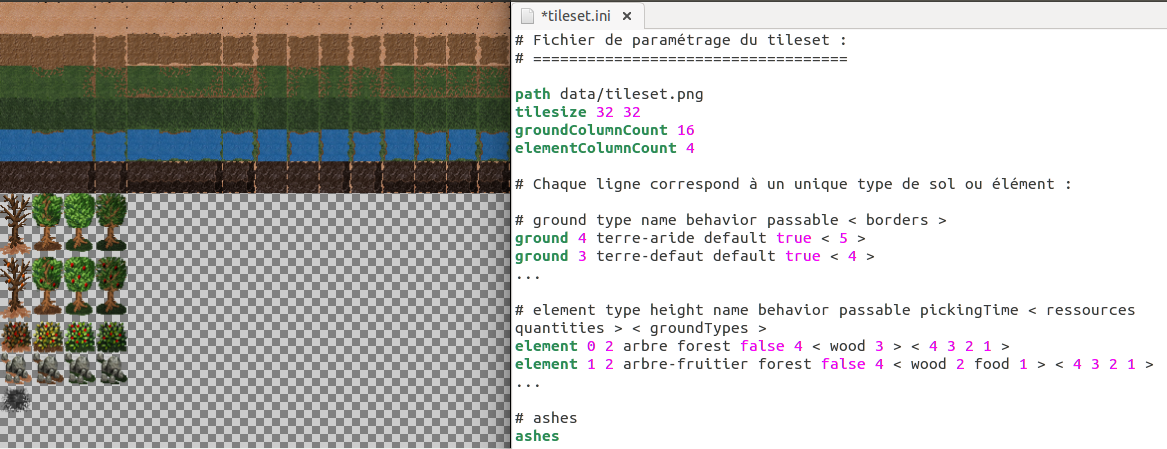
\includegraphics[scale=0.35]{img/TilesetPngIni.png}
					\end{center}
					\label{fig:tileset}
					\caption{Texture et configuration du Tileset}
				\end{figure}
				\textbf{Fichier de configuration :}\\
				Chaque ligne commençant par "\#" ne sera pas lue, ce sont les commentaires. Les mots en vert sont les mots clés utilisés pour la lecture qui se fait ligne par ligne :\\
				\begin{itemize}[label=$\bullet$]
					\item path : indique le chemin du fichier de texture du tileset\\
					\item tilesize : est suivi des dimensions (en pixel, largeur puis hauteur) d'une tuile\\
					\item groundColumnCount : nombre de colonnes pour chaque sol dans le fichier de texture (toutes les associations de rebords)\\
					\item elementColumnCount : nombre de colonnes pour chaque élément dans le fichier de texture (tous les types de sols)\\
					\item ground : définit un sol et tous ses attributs\\
					\item element : définit un élément et tous ses attributs (height est la hauteur en nombre de cases dans la texture)\\
					\item ashes : fourni une texture pour les cendres (lorsque des éléments brûlent) (cf GDD)
				\end{itemize}
				Remarque : chaque ligne commençant par ground, element ou ashes incrémente un compteur afin de connaître la position de la zone de texture correspondante. L'ordre est donc important (définition des lignes de haut en bas).\\
				\\
				\textbf{Fichier image :}\\
				Chaque ligne correspond à un type de sol ou élément.\\
				\\
				Pour chaque sol, il existe seize tuiles différentes qui correspondent à toutes les jonctions possibles avec d'autres types compatibles. Cela correspondra à l'attribut "bordures" des sols. Ils sont définis dans un ordre défini par un mot de 4 bits, avec pour chaque bit un booléen qui correspond à la présence ou non d'une bordure. En allant du bit de poids fort au bits de poids faible, on définit : gauche, bas, droite, haut.\\
				Par exemple, une bordure correspondant au mot 1111 aura des bordures tout autour tandis que celle correspondant au mot 1010 aura des bordures seulement à gauche et à droite.\\
				\\
				Pour chaque élément, il existe autant de tuiles que de types de sols compatibles. Elles sont définies dans l'ordre défini dans le fichier INI, sur une seule ligne.\\
				\\
				Enfin, il reste une ligne transparent à la fin du tileset nécessaire pour l'affichage des éléments vides.

			\subsection{Incidences}
				\label{IncidenceT}
				Ici seront brièvement expliqués les principes des différents types d'incidences environnementales, qui seront utilisées dans différentes situations.
				
				\subsubsection{Dilatation}
					Les incidences basées sur la dilatation des zones prennent en compte les types de sols ou éléments afin d'élargir les étendues voulues en propageant les sols si besoin afin de garder les contraintes définies dans le GDD.\\
					Quelques présentations des résultats de ces dilatations sont présentes en annexe, page \pageref{fig:dilatation}.
				
				\subsubsection{Erosion}
					Les incidences basées sur l'érosion des zones prennent en compte les types de sols ou éléments alentours afin de choisir les types en propageant les sols si besoin afin de garder les contraintes définies dans le GDD.\\
					Quelques présentations des résultats de ces érosions sont présentes en annexe, page \pageref{fig:erosion}.
				
				\subsubsection{Aléatoire}
					Les dernières incidences concernant le territoire sont basées sur un choix aléatoire de cases. Il s'agit ici d'appartition ou disparition de certaines ressources.\\
					Quelques présentations des résultats de ces incidences particulières sont présentes en annexe, page \pageref{fig:aleatoire}.
			
			\subsection{Gestion des contraintes}
				Comme expliqué dans la section \ref{TilesetDev}, le fichier de configuration du tileset implique une certaine quantité de contraintes de jonctions entre les sols. Par exemple, l'eau ne peut pas être juste à coté d'une falaise.\\
				Cet aspect que nous avons choisi de ne pas "coder en dur" a posé beaucoup de problèmes lors de l'utilisation de fonctions telles que changer un sol, dilater une zone, etc... (cf sections \ref{Pouvoirs}, page \pageref{Pouvoirs} et \ref{IncidenceT} ci-dessus).\\
				En effet, des fonctions ont dû être ajoutées pour comparer des sols ou connaître leurs compatibilités. De plus, chaque fonction changeant au moins un sol doit pouvoir propager les types de sols compatibles aux alentours, afin de garder une homogénéité des contraintes sur la carte. Ainsi, lorsque de l'eau est posée sur une falaise, autour de l'eau seront posés récursivement les types compatibles allant vers le type falaise :\\
				\begin{figure}[H]
					\begin{center}
						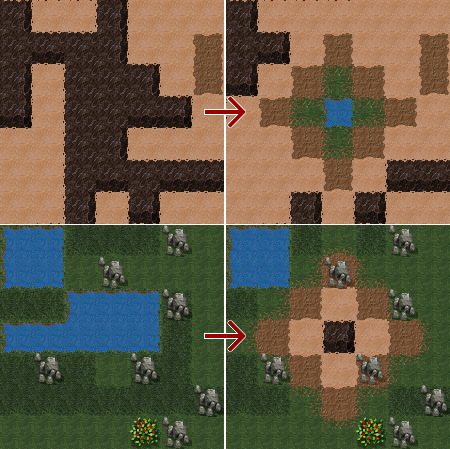
\includegraphics[scale=0.5]{img/spreadGround.png} 
					\end{center}
					\label{fig:spread}
					\caption{Exemple de propagation des contraintes sur les sols}
				\end{figure}
				Enfin, après tous les changements de sols, il faut rafraîchir les bordures de chaque case concernée afin de respecter les différentes possibilités du tileset (seize tuiles différentes, une pour chaque bordure possible ; cf section \ref{TilesetDev}, page \pageref{TilesetDev}).\\
				\\
				En conclusion, le plus difficile à gérer dans cette partie a été les précautions à prendre pour ne pas avoir de sols incompatibles entre eux, afin de garder non seulement les règles du jeu mais également l'esthétique.

		\section{Moteur multi-agent}
			Le moteur a été réalisé suivant notre propre idée de la gestion d'un systeme multi-agent après une documentation sur le sujet. 
			Les entites sont donc implémenté plus simplement que sur un moteur classique, avec uniquement les fonctionnalités indispensables, par exemple les entites ne peuvent pas communiquer entre elles.
			
			\subsection{Gestion des entités}
				Une entité est gere de maniere très basique, elles ne possedent qu'une santé discrete et un metier qui defini leurs actions.
				
				\subsubsection{La santé des entités vivantes}
					Chacune des entités possède une gestion de la santé avec plusieurs états.
					\begin{itemize}[label=$\bullet$]
						\item \textbf{Bonne santé :} Si l'entité est un citoyen, elle offre de plus grands bonus de PI.
						\item \textbf{Normal :} L'entité est dans son état par défaut.
						\item \textbf{Blessé/Malade/Fatigué :} L'entité agit avec un léger malus de vitesse. Si l'entité est un citoyen, elle offre de plus petits bonus de PI.
						\item \textbf{Gravement blessé/malade :} L'entité agit avec un malus de vitesse plus important. Si l'entité est un citoyen, elle n'offre plus de PI.
						\item \textbf{Mort :} L'entité disparaît.
					\end{itemize}
					
				\subsubsection{Incidences}
					\label{IncidenceE}
					La météo influe sur les entités en fonction de la valeur de la jauge.
					\begin{itemize}[label=$\bullet$]
						\item \textbf{Jauge positive (un ou plusieurs jours de temps ensoleillé consécutifs) :} Améliore la pousse des champs mais un excès de soleil assèche les terres et récoltes, peut réduire les étendues d'eau, une sécheresse trop longue peut faire brûler certaines ressources et augmenter la probabilité de fatigue .
						\item \textbf{Jauge négative (un ou plusieurs jours de temps pluvieux consécutifs) :} Permet de faire pousser les champs. Un surplus de pluie innonde les terres et récoltes, augmente les probabilités de maladie et peut augmenter la taille des étendues d'eau.
					\end{itemize}
					L'état de santé joue un rôle capital au niveau de la vitesse de déplacement, du temps de récolte et aussi sur la fréquence à laquelle une entité va vous apporter des points d'incidences(PI).\\
					Un état de santé faible , une maladie ou un état très faible peut entraîner le décès    d'une entité avec une probabilité de plus en plus forte dans ce même ordre de citation.\\
					Aussi chaque entité a une légère chance de donner naissance à un petit.
			
			\subsection{Gestion des scripts}
				Les scripts LUA implementent les différents comportements de toutes les catégories d'entités. Nous avons utilisé une librairie LUA permettant de redéfinir des méthodes de classe implémenté en C++ et de définir des methodes dans les classes C++ qui pourront etre appelé par les script LUA.\\
				On utilise donc un script LUA pour redifinir une methode de la classe "Entity" qui sera appelé pour simuler l'intelligence de l'entités.\\
				Par contre, cette librairie et les mécanismes de c++ nous ont imposé certaines contraintes. La plus importante est qu'il est impossible que 2 instances d'une même classe posséde 2 définissions différentes d'une de leurs methodes. Il nous a donc fallu implémenter une sous-classe pour chaque catégorie d'entités afin d'avoir un comportement different pour toutes ces categories. Cette problematique empeche les joueurs de pouvoir créer de nouvelles catégories d'entite, il pourra cependant modifier celle deja existante.
				
			\subsection{Liste des scripts}
				Le comportement des agents, en ce qui concerne le déplacement, a soulevé le problème de la gestion des obstacles étant donné que certains éléments du décor ne sont pas franchissables.\\
				En effet, certaines actions nécessitant un trajet spécifique utilisent le résultat d'un algorithme de recherche de chemin et se déroulent sans interruption sur plusieurs ticks, c'est-à-dire sans rappeler le script de l'agent.\\
				Par conséquent, les directives des scripts sont en partie des objectifs à atteindre et non de simples actions isolées.
	
				\subsubsection{Les citoyens alliés}
					\begin{itemize}[label=$\bullet$]
						\item \textbf{Récolteurs(bûcherons, cueilleurs, mineurs) :} \\ Si un bûcheron faible, un mineur faible ou un cueilleur perçoit un animal agressif ou un citoyen ennemi celui-ci va fuir.\\
							Si un bûcheron ou un mineur se fait attaquer, il va répliquer en attaquant en priorité l'entité face à lui si celle-ci l'attaque.\\
							A chaque fois que l'entité récolte une ressource elle remplit son sac puis se dirige vers la base pour la déposer.\\
							Lorsque son sac est vide, elle regarde dans son rayon de perception si une ressource est disponible. Si au moins une ressource est repérée, elle se dirige vers la plus proche pour la récolter. Sinon, elle se dirige de manière aléatoire.
						\item \textbf{Chasseurs :} \\ Le chasseur reste relativement proche de la base et adopte un rôle de défenseur.\\
							S'il est attaqué, il va regarder le nombre de chasseurs et le nombre d'entités hostiles autour de lui , s'il y a moins d'entités hostiles que de chasseurs auxquels on ajoute 3, il va attaquer l'entité qui l'attaque avec dans l'ordre de priorité : l'entité en face de lui, un citoyen ennemi et un animal agressif. Sinon il adopte la fuite.\\
							S'il n'est pas attaqué, tout en gardant une distance proche de la base ,il va chercher une cible autour de lui dans cet ordre de priorité, un citoyen ennemi, un animal agressif puis un animal passif.\\
							Encore une fois s'il n'y a pas trop d'ennemis aux alentours, le chasseur va aller attaquer la cible sinon il va fuir.\\
							S'il n'y a ni citoyens ennemis ni animaux autour de lui et s'il n'est pas trop loin de la base, il va avancer aléatoirement sinon il va revenir vers la base.
					\end{itemize}
		
				\subsubsection{Les citoyens ennemis}
					Les citoyens ennemis ont un comportement agressif.\\
					S'ils sont attaqués, il vont adopter le même comportement qu'un chasseur sauf que dans l'ordre de priorité ils vont attaquer: l'entité en face d'eux, un chasseur et un récolteur.\\
					S'ils ne sont pas attaqués, même démarche que le chasseur en changeant l'ordre de priorité par un chasseur puis un récolteur.\\
					Si aucun chasseur ou récolteur n'est perçu dans leurs rayons de perception, ils vont avancer aléatoirement.
			
				\subsubsection{Les animaux}
					\begin{itemize}[label=$\bullet$]
						\item \textbf{Agressifs :} \\
							Dès qu'un animal agressif perçoit une entité excepté un animal agressif il va l'attaquer, en attaquant en priorité l'entité qui est en face de lui. Si aucune entité n'est perçue ou s'il ne perçoit que des animaux agressifs , l'animal va se déplacer aléatoirement.
						\item \textbf{Passifs :} \\
							L'animal passif va tout simplement fuir toutes les entités à l'exception des animaux passifs.
					\end{itemize} \normalsize 

				Dans certaines situations vues précédemment, l’entité se déplacera de manière aléatoire et pourra marquer un arrêt de temps à autre afin de simuler un comportement naturel.
	
		\section{Météo}
			La météo est gérée comme une jauge comprise entre cinq et moins cinq. Au commencement d'une partie la jauge est à zéro.\\
			A la fin de chaque journée nous comparons le temps du jour terminé avec le temps du jour précédent, si celui-ci est le même et est ensoleillé la jauge augmente , si par contre le temps est pluvieux la jauge descend.\\
			En revanche, si la jauge est entre -3 et -5 et que la journée fut ensoleillé ou inversement si la jauge est entre 3 et 5 et qu'il fit un temps pluvieux la jauge revient respectivement à -1 ou 1.\\
			Plus la valeur de la jauge est grande positivement ou négativement, plus il y aura d'incidences en rapport avec la pluie pour les valeurs négatives et inversement pour le soleil.
	
		\section{Architecture}
			L'application est composée de plusieurs états représentant les menus et la partie entre lesquels il est possible de naviguer.
			
			\subsection{Main menu state}
				Le menu principal est le premier état de l’application, il sert d’écran d’accueil et dispose de trois boutons :
				\begin{itemize}[label=$\bullet$]
					\item "Start" qui crée une nouvelle instance de jeu et appelle l’état "Game State".
					\item "Load" qui appelle l’état "Load Menu State".
					\item "Exit" qui quitte l’application.
				\end{itemize}
				
			\subsection{Game state}
				L’état de jeu est le primordial au sein de l’application, il sert de support à l’instance de jeu afin d’en gérer le déroulement. Il contient l’affichage de la partie visible de la carte du monde et des entités ainsi qu’une interface, permettant au joueur de gérer la partie, ayant deux fonctions. La première consiste à informer de la valeur de certaines variables inhérentes à la partie comme le nombre de points ou d’une certaine ressource. La seconde permet au joueur d’indiquer les actions qu’il souhaite réaliser via un ensemble de boutons.
				
			\subsection{Night state}
				L’état de nuit revient régulièrement au cours de la partie, pendant celui-ci ont lieu les incidences sur le territoire (cf section \ref{IncidenceT}, page \pageref{IncidenceT}) et sur les entités (cf    section \ref{IncidenceE}, page \pageref{IncidenceE}).\\
				De plus, cet état permet au joueur de déterminer directement la météo de la prochaine journée de jeu et d’influer indirectement sur les proportions des rôles des entités. En plus de cela, un bouton de validation supprime l’état courant afin que la partie puisse reprendre son cours dans l’état de jeu.
				
			\subsection{End state}
				L’état de fin de partie signale au joueur qu’il a atteint la condition de défaite, il dispose simplement d’un bouton :
				\begin{itemize}[label=$\bullet$]
					\item "Back" qui supprime l’état courant.
				\end{itemize}
				
			\subsection{Game menu state}
				Le menu de jeu est l’état de pause du jeu, il dispose de quatre boutons :
				\begin{itemize}[label=$\bullet$]
					\item "Back" qui supprime l’état courant.
					\item "Save" qui appelle l’état "Save Menu State".
					\item "Load" qui appelle l’état "Load Menu State".
					\item "Quit" qui supprime tous les états jusqu’à l’état "Main Menu State".
				\end{itemize}
				
			\subsection{Save menu state}
				Le menu de sauvegarde est l’état qui permet de sauvegarder son avancement, il dispose d’un champ de saisie du nom de sauvegarde et de deux boutons :
				\begin{itemize}[label=$\bullet$]
					\item "Back" qui supprime l’état courant.
					\item "Save" qui crée un fichier de sauvegarde à partir de l’instance de jeu en cours et le nomme d’après le texte entré.
				\end{itemize}
				
			\subsection{Load menu state}
				Le menu de chargement est l’état qui permet de charger une partie précédemment sauvegardée, il dispose d’une liste de boutons, représentant les fichiers de sauvegarde répertoriés à partir desquels l’instance de jeu sera modifiée, de deux boutons permettent de parcourir la liste et d’un dernier bouton :
				\begin{itemize}[label=$\bullet$]
					\item "Back" qui supprime l’état courant.
				\end{itemize}
			
	\chapter{Post-Mortem}
		Cette section liste toutes les étapes de la conception que nous n'avons pas réalisées (selon notre ordre de priorités), ainsi que toutes les améliorations auxquelles nous avons pensé lors de la phase de développements.
		
		\section{Fonctionnalités non implémentées}
			Tous les bâtiments sont réalisables mais nous n'avons pas implémenté la possibilité pour les entités de construire des bâtiments par conséquent le bois et la pierre n'ont encore aucune utilité. 
			
			% animation ?
			
			Une des fonctionnalité majeur non-implémenté est la gestion d'un arbre technologique, qui mettrait de debloquer de nouveaux batiments mais aussi de diminuer le temps de récolte des ressources en déverrouillant différentes technologies. Chacune d'elles coûterait une certaine quantité de bois, de pierre et de nourriture. 
			
			Certains pouvoirs divins n'ont pas été mis en place, comme le soin des citoyens du joueur ou bien la création d'une entités en cours de journée. 
			
			Le karma, reflètant l'équilibre entre "bonnes" et "mauvaises" actions et se répercutant sur le comportement des entités quant à l'appel d'un "bon" ou d'un "mauvais" script, est une autre fonctionnalité non ajoutée.
			
		\section{Améliorations réalisables}
			Au niveau de la carte, il serait possible de créer un éditeur de carte, sachant que toute les fonctions nécessaires existent déjà. Nous pourrions également modifier la génération aléatoire de carte pour avoir des cartes plutôt arides ou plutôt humides par exemple.
			De plus, une indication visuelle indiquant le coût et la possibilité ou non de placer un sol ou un element sur la carte, via les pouvoirs du joueur, est une amélioration que nous souhaitons rapidement implémenter.
			
			Une diversification des espèces pour les animaux nous permettrait ainsi d'ajouter la notion de troupeau afin de se rapprocher le plus fidèlement d'un comportement naturel.
			Le troupeau serait dirigé par un chef  et les entités le constituant attaqueraient et se défendraient en groupe.
			Ceci permettrait d'avoir une intéraction entre les animaux d'une
			même espèce et entre ceux venant d'espèces différentes.
			
			
			Les civilisations "neutres" ont aussi été abordé, celles-ci seraient composées d'entités possiblement alliées et permettraient, par exemple, des échanges de ressource ainsi qu'un système d'interactions entre les civilisations, à l'intérieur ou en dehors des limites de la carte (nous pouvons imaginer des émissaires étrangers venant commercer par exemple).
			
			Le jeu n'a pour l'instant aucune condition de victoire, la partie se terminé qu'en cas de défaite, nous souhaitons ajouter différentes conditions de victoire. Ceci nous permettrait ainsi de mettre en place plusieurs mode de jeu, un libre qui est le seul mode jouable actuellement mais aussi un mode campagne avec plusieurs objectifs à atteindre tout le long de cette campagne. Les conditions de victoire pourrait être d'atteindre un certain point sur la carte, de récolter un nombre definit de ressource ou bien la construction d'un certain nombre de bâtiment spécifique.
			
			Au niveau de l'interface, nous pourrions mettre en place du son (musiques et bruitages), avoir un système de statistiques pour comparer les résultats de différentes parties.
			Nous pourrions aussi %TODO
	
	\appendix
	\chapter{}
		Dans cette partie seront placés les éléments trop volumineux pour être inclus directement dans le texte, tels que les images ou graphiques.\\
		
		\section{Diagramme de Gantt}
			Le diagramme est fourni page \pageref{fig:gantt}.
			
		\section{Comparatif de performances}
			Le graphique est situé page \pageref{fig:analyse}.
			
		\section{Incidences sur la carte}
			Les présentations sont présentes de la page \pageref{fig:dilatation} à la page \pageref{fig:aleatoire}.
			
		\section*{}
			\begin{figure}
				\vspace{-3,5cm} \hspace{-4,5cm} 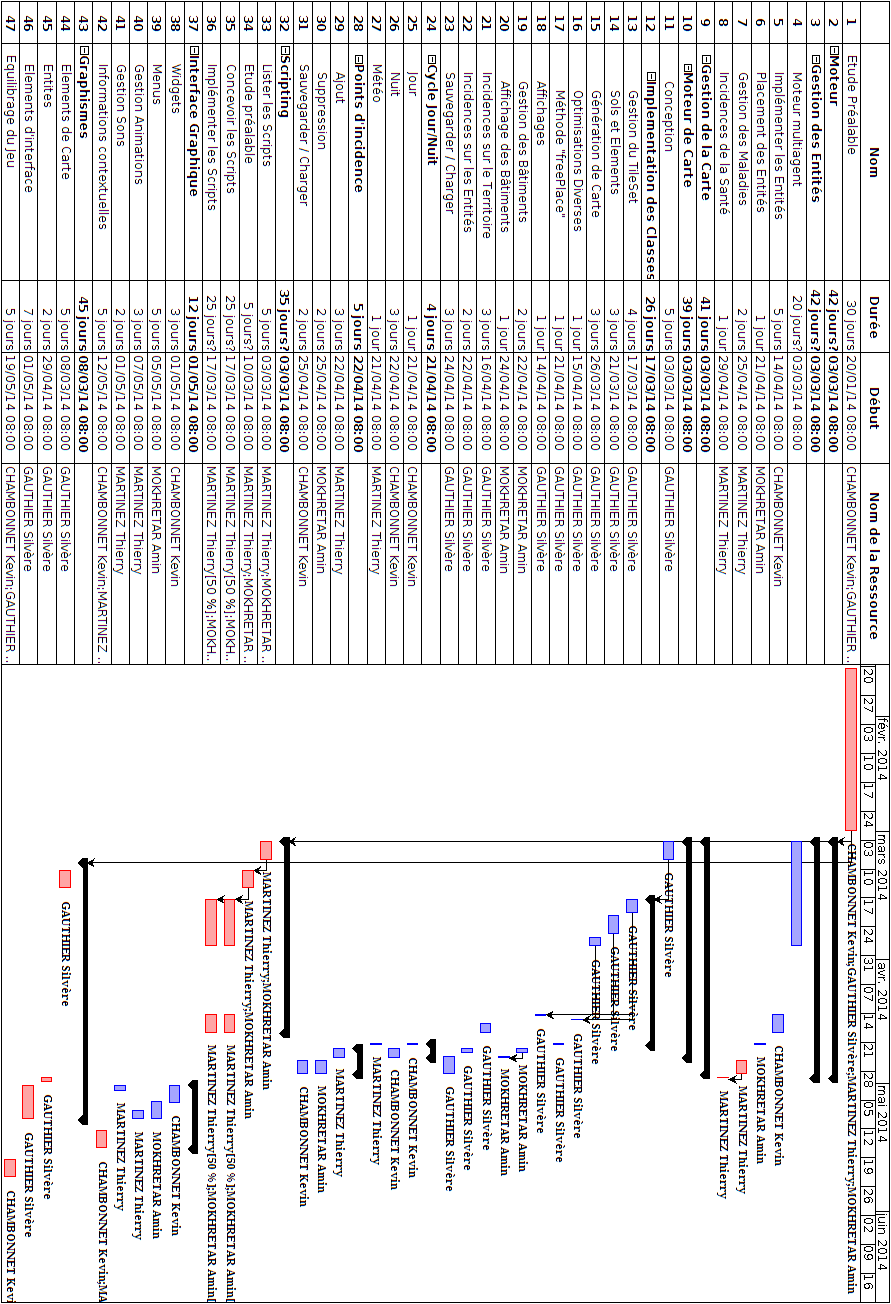
\includegraphics[scale=0.6]{img/Gantt.png}
				\label{fig:gantt}
				\vspace{-0,5cm} \caption{Diagramme de Gantt}
			\end{figure}
			
			\begin{figure}
				\begin{center}
					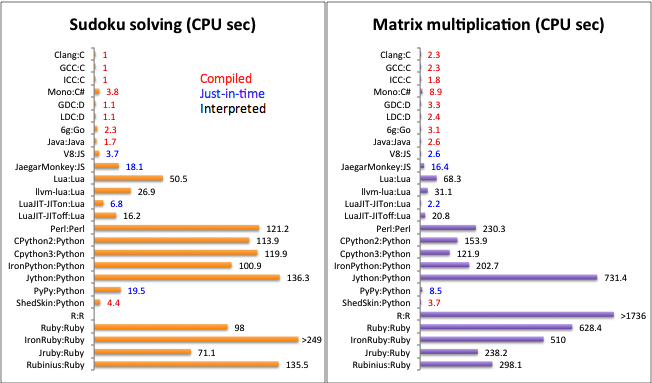
\includegraphics[scale=0.5]{img/AnalyseLangage1.png}
					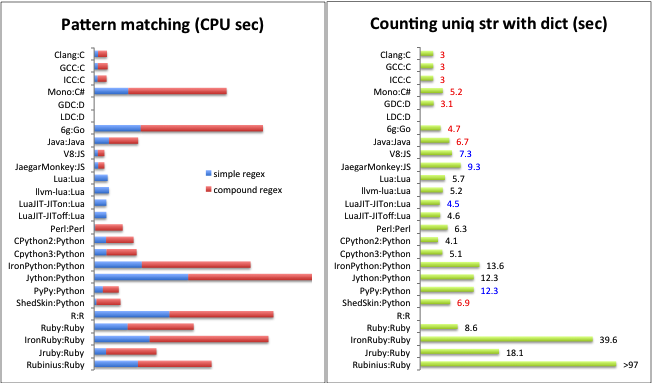
\includegraphics[scale=0.5]{img/AnalyseLangage2.png} 
				\end{center}
				\label{fig:analyse}
				\caption{Comparaisons de performances de divers langages dans des cas donnés}
			\end{figure}
			
			\begin{figure}
				\begin{center}
					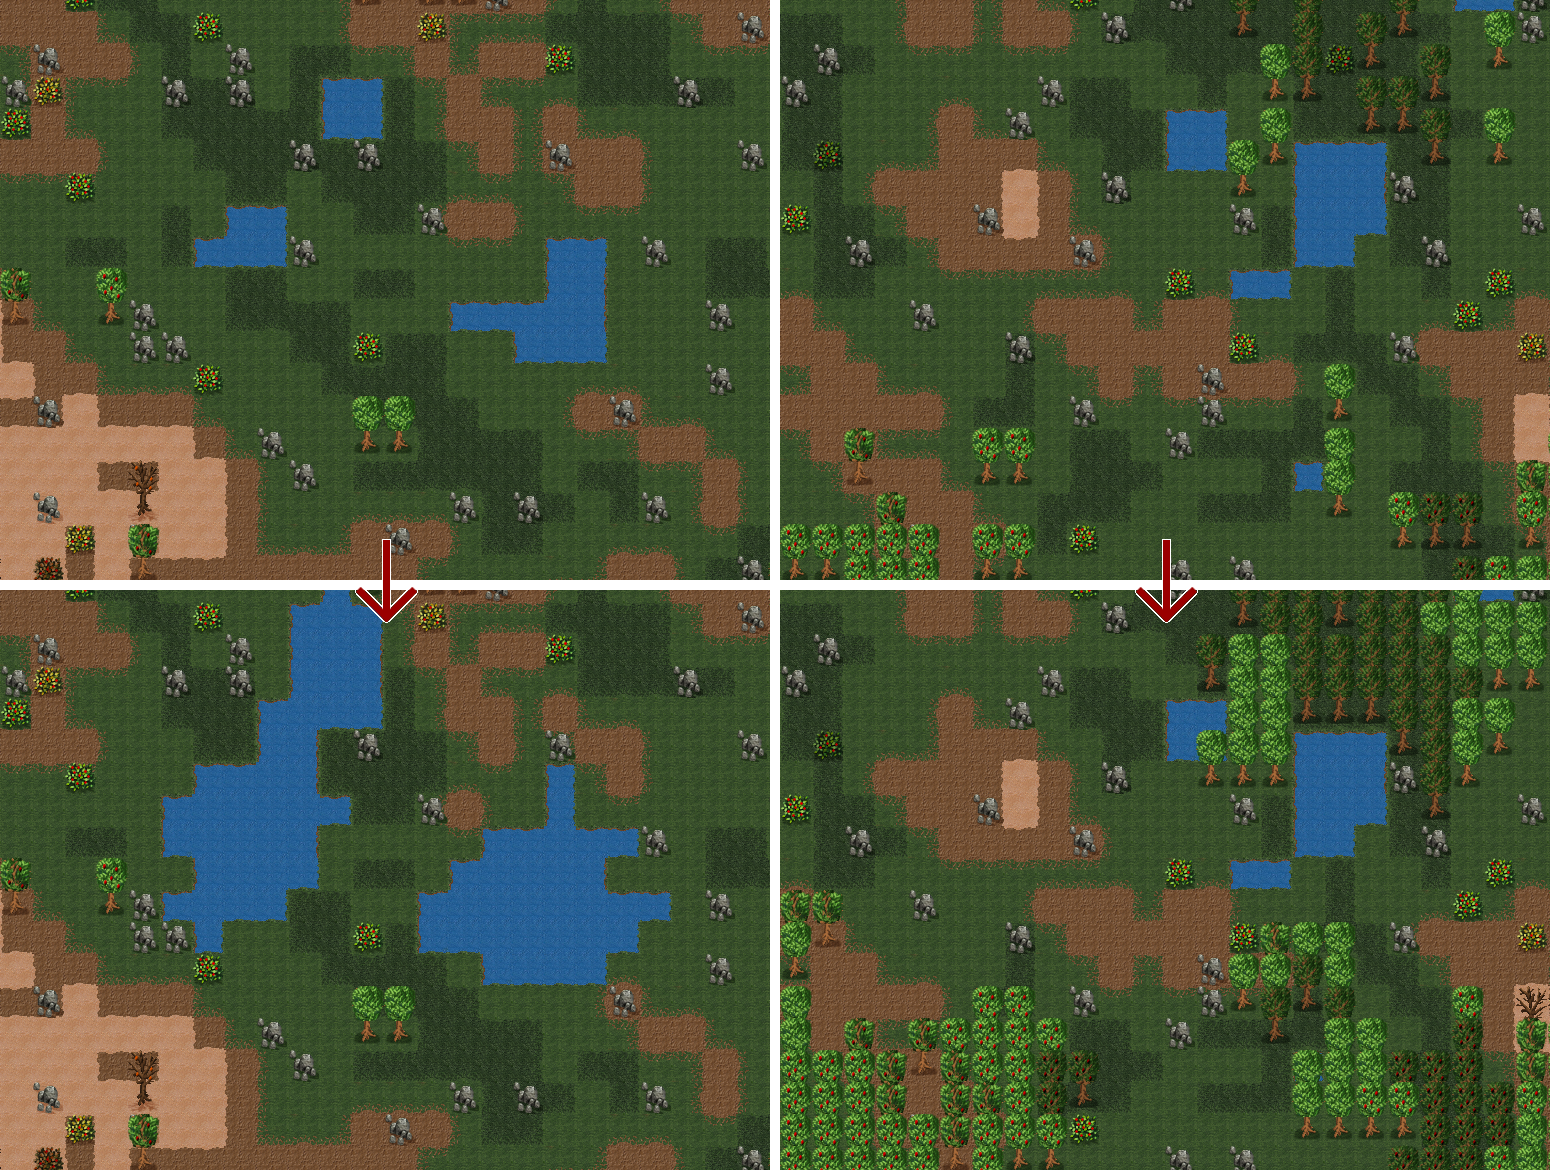
\includegraphics[scale=0.2]{img/Dilatation.png}
				\end{center}
				\label{fig:dilatation}
				\caption{Dilatations après trois itérations}
			\end{figure}
			\begin{figure}
				\begin{center}
					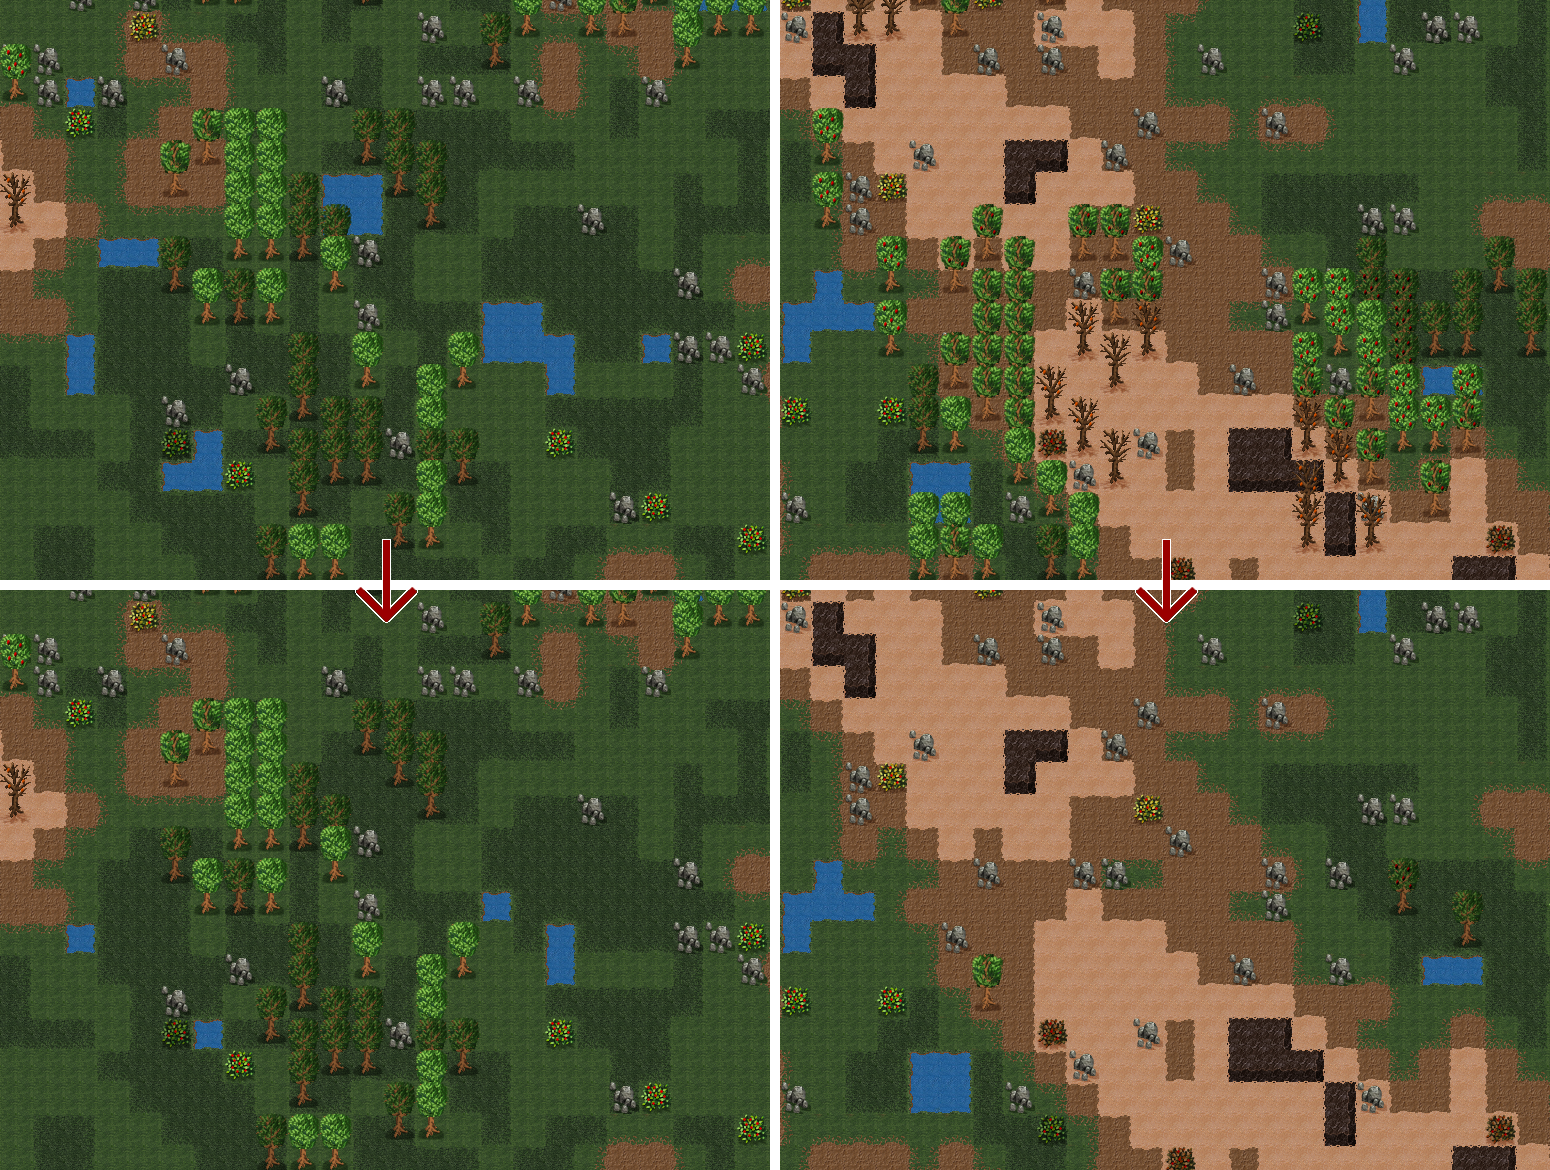
\includegraphics[scale=0.2]{img/Erosion.png}
				\end{center}
				\label{fig:erosion}
				\caption{Erosions après trois itérations}
			\end{figure}
			\begin{figure}
				\begin{center}
					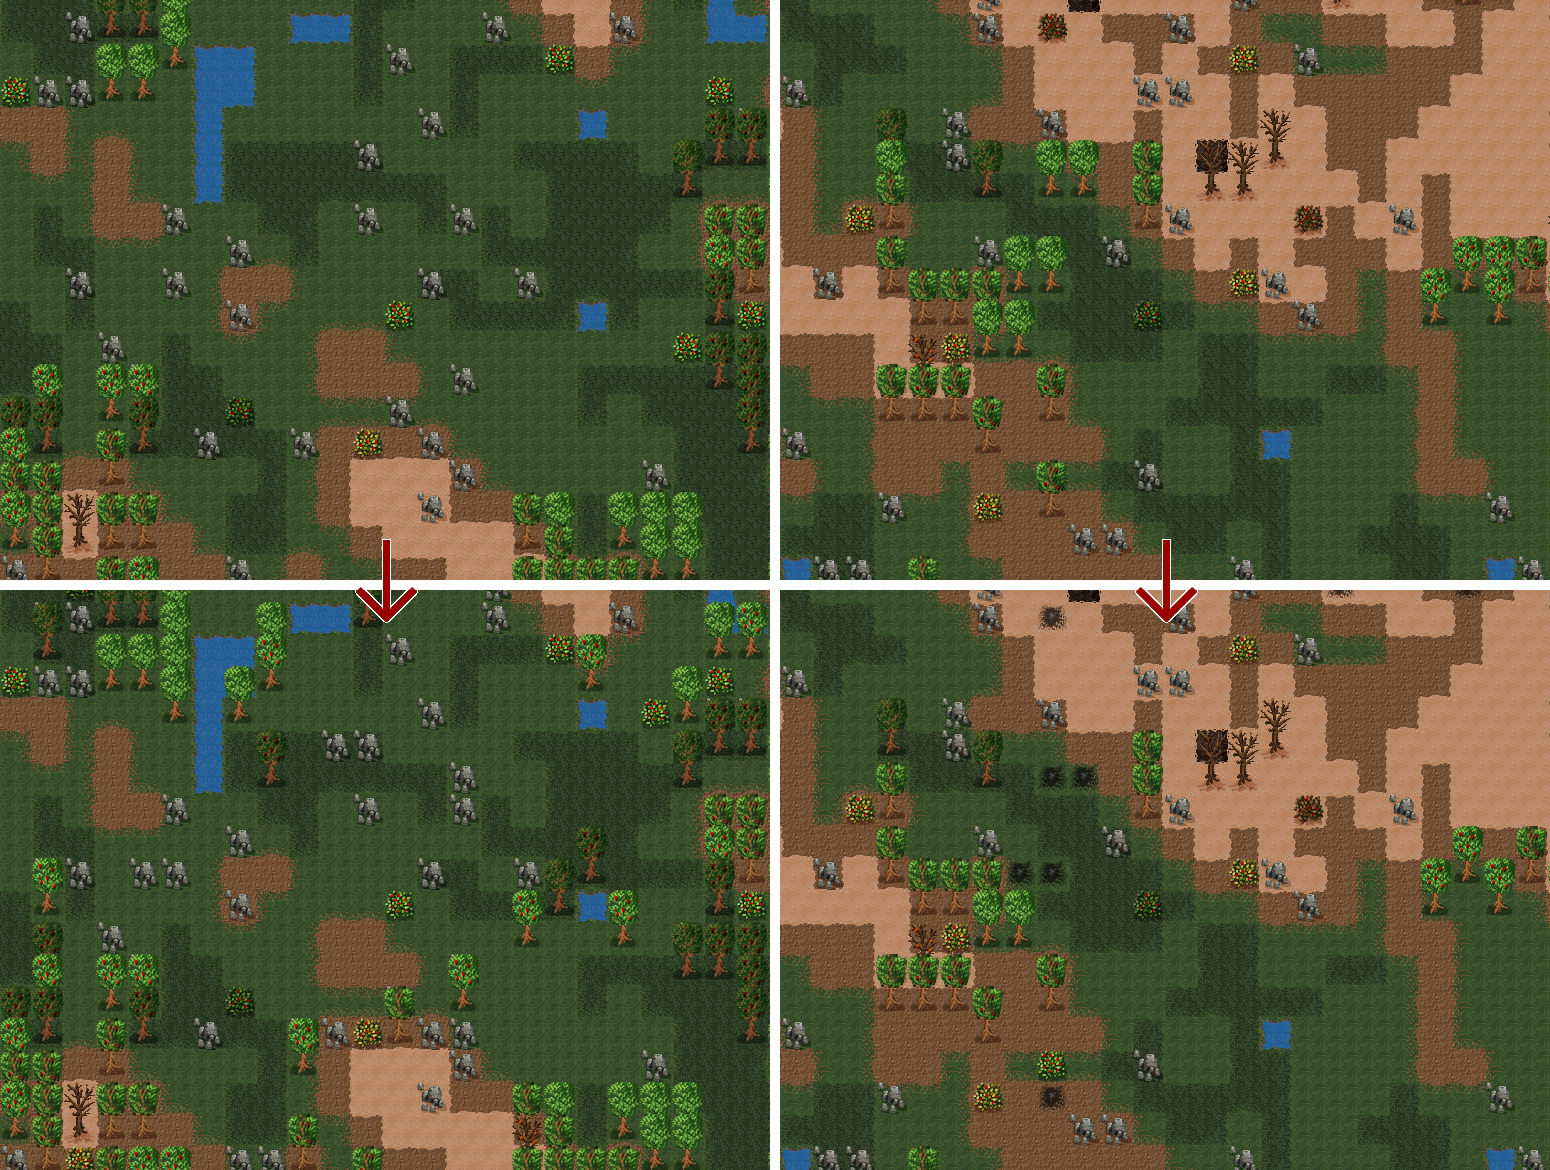
\includegraphics[scale=0.2]{img/Aleatoire.png}
				\end{center}
				\label{fig:aleatoire}
				\caption{Aléatoires après trois itérations}
			\end{figure}

\end{document}
